\let\negmedspace\undefined
\let\negthickspace\undefined
\documentclass[journal,12pt,twocolumn]{IEEEtran}
\usepackage{cite}
\usepackage{amsmath,amssymb,amsfonts,amsthm}
\usepackage{algorithmic}
\usepackage{graphicx}
\usepackage{textcomp}
\usepackage{xcolor}
\usepackage{txfonts}
\usepackage{listings}
\usepackage{enumitem}
\usepackage{mathtools}
\usepackage{gensymb}
\usepackage{comment}
\usepackage[breaklinks=true]{hyperref}
\usepackage{tkz-euclide} 
\usepackage{listings}
\usepackage{gvv}                                        
\def\inputGnumericTable{}                                 
\usepackage[latin1]{inputenc}                                
\usepackage{color}                                            
\usepackage{array}                                            
\usepackage{longtable}                                       
\usepackage{calc}                                             
\usepackage{multirow}                                         
\usepackage{hhline}                                           
\usepackage{ifthen}                                           
\usepackage{lscape}
\setlength{\arrayrulewidth}{0.5mm}
\setlength{\tabcolsep}{18pt}
\renewcommand{\arraystretch}{1.5}

\newtheorem{theorem}{Theorem}[section]
\newtheorem{problem}{Problem}
\newtheorem{proposition}{Proposition}[section]
\newtheorem{lemma}{Lemma}[section]
\newtheorem{corollary}[theorem]{Corollary}
\newtheorem{example}{Example}[section]
\newtheorem{definition}[problem]{Definition}
\newcommand{\BEQA}{\begin{eqnarray}}
\newcommand{\EEQA}{\end{eqnarray}}
\newcommand{\define}{\stackrel{\triangle}{=}}
\theoremstyle{remark}
\newtheorem{rem}{Remark}
\begin{document}


\title{Waves(20) 11.15}
\author{EE23BTECH11051-Rajnil Malviya}
\date{January 2024}



\maketitle

\subsection*{\textbf{Question :-}}
A train, standing at the outer signal of a railway station blows a whistle of frequency
400 Hz in still air. (i) What is the frequency of the whistle for a platform observer
when the train (a) approaches the platform with a speed of $10 ms^{-1} $, (b) recedes
from the platform with a speed of $10 ms^{-1} $? (ii) What is the speed of sound in each
case ? The speed of sound in still air can be taken as $340 ms^{-1} $.

\bigskip
 This problem requires knowledge of \textit{Doppler Effect} , So first we will learn Doppler effect and then we will solve our problem . Before learning Doppler effect , we will also understand Sound Waves .

\subsection*{\textbf{Equation of Sound Wave :-}}
Sound Wave is transmission of energy ; sound wave depends on many parameters . A general equation of sound wave is shown below 
\begin{align}y(t) = Asin( 2 \pi ft + \phi ) \end{align} 
\textit{y(t) is instantaneous 
displacement of wave at time t;}$$\textit{A is amplitude of wave;}$$$$f\;is\; frequency\; of\; wave;$$
$$t \;is\; time;$$$$\phi \; is \; phase \; angle;$$
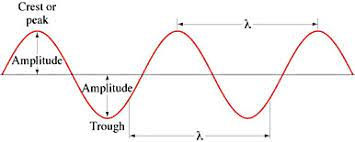
\includegraphics[width=0.45\textwidth]{figs/waves.jpeg}\\
$$\lambda \;is\; wavelength\; of\; wave;$$$$crest \;is\; peak(highest\; point) \;of\; wave;$$$$trough\; is\; dip(lowest\; point) \;of\; wave;$$
$$2\pi f \;is \; called\; angular frequency;$$

On comparing our problem with equation (3) , equation for different cases are given\\\\
$equation \;of\; sound\; wave\; when\; whistle\; is\; blown\; by$
\textit{train is}
$$y(t) = Asin( 2 \pi \times400\times t + \phi ) $$ 
\;\;\;\;\;\;\;\;\;\;\;\;\;\;\;\;\;\;\;\;for this case $f\;=\;400Hz$\\\\
$equation \;of\; sound\; wave\; observed\; by\; observer\;when\\ \;train\;is\; approaching\; observer\;$
$$y(t) = Asin( 2 \pi \times412.1212\times t + \phi ) $$ 
\;\;\;\;\;\;\;\;\;\;\;\;\;\;\;\;\;\;\;\;for this case $f\;=\;412.1212Hz$\\\\
$equation \;of\; sound\; wave\; observed\; by\; observer\;when\\ \;train\;is\; receding\; observer\;$
$$y(t) = Asin( 2 \pi \times388.5714\times t + \phi ) $$ 
\;\;\;\;\;\;\;\;\;\;\;\;\;\;\;\;\;\;\;\;for this case $f \;\;= \;\;388.5714Hz$\\
\subsection*{\textbf{Doppler Effect for Sound Waves :-}}
Doppler effect for sound wave refers to change in frequency or pitch of sound wave observed by an observer when there is a relative motion between observer and source .\\\\

    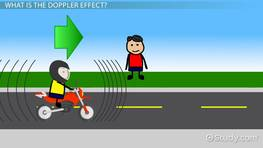
\includegraphics[width=0.89\linewidth]{figs/doppler.jpg}\\\\

\subsection*{\textbf{Derivation \;of \;Doppler :-}}
To derive Doppler , we can write equation of sound as shown
\begin{align}f = \frac{v}{\lambda}\end{align}
using equation (2) , we get
\begin{align}y(t) = Asin( 2 \pi \frac{v}{\lambda}t + \phi ) \end{align}  
$$v \;is\; speed\; of\; sound\; in\; that\; medium$$
\textbf{1.} Source is moving toward stationary Observer-\\\\
Now consider the relative motion in which source is moving towards observer , in that case effective wavelength $\lambda'$ observed by observer will be compressed ,
$$v_s \;is\; velocity\; of\; source$$
$$v_o \;is\; velocity\; of\;observer $$
$$v_s = v_s$$
$$v_o = 0$$
\begin{align}\lambda' = \lambda - v_s T\end{align}
T is time period(time taken by source wave to complete one revolution)
and effective frequency \textit{f}' observed by observer will be
\begin{align}f' = \frac{v}{\lambda'}\end{align}
using equations (2) , we get
\begin{align}f' = \frac{v}{\lambda- v_s T}\end{align}
$$f' = \frac{v f}{f(\lambda- v_s T)}$$
we know ,
\begin{align}T = \frac{1}{f}\end{align}
using equation (7)
\begin{align}f' = \frac{v f}{v- v_s }\end{align}
\bigskip\\
\textbf{2.} Source is moving away from stationary Observer-\\\\
Similarly , if source is receding from observer than $\lambda, $will be increased
$$v_s = v_s$$
$$v_o = 0$$
\begin{align}\lambda' = \lambda + v_s T\end{align}
using equations (5) and (9) , we get
\begin{align}f' = \frac{v}{\lambda+ v_s T}\end{align}
$$f' = \frac{v f}{f(\lambda+v_s T)}$$
using equation (2) and (7)
\begin{align}f' = \frac{v f}{v+ v_s }\end{align}
\textit{Doppler effect depends on relative velocity }, so we will use this concept to prove frequencies for different cases depending on situation .\\\\
\textbf{3.} Observer is moving towards Stationary Source-\\\\
In this case , the velocity at which sound is approaching observer will increase .
$$v_s = 0$$
$$v_o = v_o$$
\begin{align}f' = \frac{v'}{\lambda'}\end{align}
\begin{align}v'= v+v_o\end{align}
$$But \;what\; about\; wavelength??$$
It's answer is , wavelength will be same  .\\

    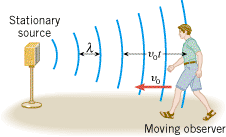
\includegraphics[width=0.9\linewidth]{figs/wave3.png}\\\\
Sound properties only depends on situation of source and not observer .
\begin{align}\lambda' = \lambda\end{align}
using equations (13) and (14) , and substituting in equation (12) 
\begin{align}f' = \frac{v+v_o}{\lambda}\end{align}
using equation (2) , we get 
\begin{align}f' = \frac{(v+v_o) f}{v }\end{align}
\textbf{4.} Observer is moving away from Stationary Source-\\\\
In this case , the velocity at which sound is approaching observer will decrease .
$$v_s = 0$$
$$v_o = v_o$$
\begin{align}v'= v-v_o\end{align}
In this case also , wavelength will not change.
\begin{align}\lambda' = \lambda\end{align}
using equations (17) and (18) , and substituting in equation (12) 
\begin{align}f' = \frac{v-v_o}{\lambda}\end{align}
using equation (2) , we get 
\begin{align}f' = \frac{(v-v_o) f}{v }\end{align}\\
\textbf{5.} Source and Observer are both moving towards each other-\\\\
In this case , the velocity at which sound is approaching observer will increase and wavelength will compress .
$$v_s = v_s$$
$$v_o = v_o$$
\begin{align}v'= v+v_o\end{align}
\begin{align}\lambda' = \lambda - v_s T\end{align}
using equations (21) and (22) , and substituting in equation (12) 
\begin{align}f' = \frac{v+v_o}{\lambda-v_s T}\end{align}
using equation (2) , we get 
\begin{align}f' = \frac{(v+v_o) f}{v-v_s }\end{align}
\textbf{6.} Source and Observer are both moving away from each other-\\\\
In this case , the velocity at which sound is approaching observer will decrease and wavelength will stretch .
$$v_s = v_s$$
$$v_o = v_o$$
\begin{align}v'= v-v_o\end{align}
\begin{align}\lambda' = \lambda + v_s T\end{align}
using equations (25) and (26) , and substituting in equation (12) 
\begin{align}f' = \frac{v-v_o}{\lambda+v_s T}\end{align}
using equation (2) , we get 
\begin{align}f' = \frac{(v-v_o) f}{v +v_s}\end{align}
\textbf{7.} Source is moving towards Observer and Observer moving away from Source-\\\\
In this case , the velocity at which sound is approaching observer will decrease and wavelength will compress .
$$v_s = v_s$$
$$v_o = v_o$$
\begin{align}v'= v-v_o\end{align}
\begin{align}\lambda' = \lambda - v_s T\end{align}
using equations (29) and (30) , and substituting in equation (12) 
\begin{align}f' = \frac{v-v_o}{\lambda-v_s T}\end{align}
using equation (2) , we get 
\begin{align}f' = \frac{(v-v_o) f}{v -v_s}\end{align}
\textbf{8.} Source is moving away from Observer and Observer is moving towards Source-\\\\
In this case , the velocity at which sound is approaching observer will increase and wavelength will stretch.
$$v_s = v_s$$
$$v_o = v_o$$
\begin{align}v'= v+v_o\end{align}
\begin{align}\lambda' = \lambda + v_s T\end{align}
using equations (33) and (34) , and substituting in equation (12) 
\begin{align}f' = \frac{v+v_o}{\lambda+v_s T}\end{align}
using equation (2) , we get 
\begin{align}f' = \frac{(v+v_o) f}{v +v_s}\end{align}\\\\
\textbf{9.} Both Source and Observer are stationary-\\\\
If both Source and Observer are stationary , it means 
$$v_s = 0$$
$$v_o = 0$$
also there will be no change in wavelength 
\begin{align}\lambda' = \lambda\end{align}
\begin{align}v'= v\end{align}
using equation (37) and (38), and substituting in equation (12) 
\begin{align}f' = \frac{v}{\lambda}\end{align}
using equation (2) , we get 
\begin{align}f' = f\end{align}\\\\

So , Doppler effect depends on relative velocity of Observer and Source with respect to same frame and also velocity of Sound in that medium .\\\\
Let's get back to our problem solution\\\\
Solution :-\\
         \begin{table}[h]
        
\begin{tabular}{ | m{3.4em} | m{5cm} | } 
  \hline
 \textbf{Symbol} & \textbf{Meaning of Symbol}  \\
 \hline
 $f$ & actual frequency of source  \\
\hline
$f_a'$ & frequency observed by observer when train is approaching observer  \\
\hline
 $f_r'$ &  frequency observed by observer when train is receding observer  \\
\hline
 $v$ & velocity of air in that medium  \\
\hline
$v_s$ & velocity of source which is train  \\
\hline
$v_o$ & velocity of observer  \\
\hline
\end{tabular}

    \end{table}

(i)  a. When the train approaches the platform (i.e., the observer at rest), so this situation is similar to our \textbf{(1.)} derivation of Doppler effect , so we will use equation (8). If we compare with equation (8) which is given below
$$f' = \frac{v f}{v- v_s }$$
 \begin{table}[h]
        \begin{tabular}{ | m{3.3cm} | m{3.5cm} | }
  \hline
 \textbf{Symbol for Problem} & \textbf{ Symbol in equation 8}  \\
 \hline
 $f_o$ & $f$\\
\hline
$f_a'$ & $f'$\\
\hline
 $v$ & $v$\\
\hline
$v_t$ & $v_s$  \\
\hline
$v_o$ & $v_o$ \\
\hline
\end{tabular}
    \end{table}
On Substituting
\begin{align}f'_a=f_o\times\frac{v}{v-v_t}\end{align}

$$f'_a=400\times\frac{340}{340-10}$$

$$f'_a=412.1212$$
\bigskip

b. When the train recedes the platform (i.e., the observer at rest), it is similar to our \textbf{2.} in Doppler derivation and equation (11)
$$f' = \frac{v f}{v+ v_s }$$
$f'_r $ is frequency observed by observer when train is receding platform,\\
On comparing with equation (11) 
$$f'_r =f'$$
substituting in equation (11)
\bigskip
    \begin{table}[h]
   
        \setlength{\arrayrulewidth}{0.5mm}
\setlength{\tabcolsep}{18pt}
\renewcommand{\arraystretch}{1.5}


\begin{tabular}{ |p{2cm}|p{2cm}|p{2cm}|p{3cm}|p{1}p{1}}
    \hline
    \multicolumn{4}{|c|}{frequencies observed in Different cases} \\
    \hline
    Doppler Shift &Stationary Observer &Observer moving towards Source &Observer moving away from Source\\
    \hline
    Stationary Source & $$f' = f$$& $$f' = \frac{(v+v_o) f}{v}$$&$$f' = \frac{(v-v_o) f}{v}$$\\
    \hline
    Source moving towards Observer &$$f' = \frac{v f}{v-v_s }$$&$$f' = \frac{(v+v_o) f}{v- v_s }$$&$$f' = \frac{(v-v_o) f}{v- v_S }$$\\
    \hline
    Source moving away from Observer&$$f' = \frac{v f}{v+ v_s }$$&$$f' = \frac{(v+v_o) f}{v+ v_s }$$&$$f' = \frac{(v-v_o) f}{v+ v_s }$$\\
    \hline
    \end{tabular}

       
    \end{table}
    \newpage
    
\begin{align}f'_r=f_o\times\frac{v}{v+v_t}\end{align}

$$f'_r=400\times\frac{340}{340+10}$$

$$f'_r=388.5714$$\\
(ii) The speed of sound in each will be same.It is $340  ms^{-1}$ in each case.
We are providing a table in which various formulas of frequencies are written depending on situation .\\\\


  
\end{document}
